
As mentioned above, we classify fragmentation as being either internal or external. Internal fragmentation is considered wasted space due to alignment and it may sometimes be required for an allocator to allocate a slightly smaller block of memory than a user has requested. Figure~\ref{fig:internal_fragmentation} shows an example of when a user has requested 100 bytes, where the allocator has allocated 128 bytes instead due to alignment. In this case, the last 28 bytes are wasted space since the user will not use them.

\begin{figure}[H]
    \centering
    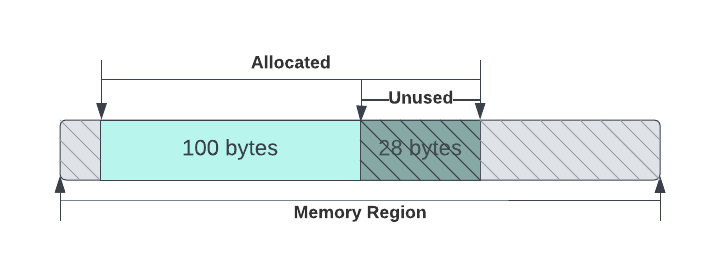
\includegraphics[width=0.75\textwidth]{figures/internal_fragmentation.png}
    \caption{A memory region containing one allocated piece of memory that is 128 bytes large. However, the user only requires 100 bytes of those and thus, 28 bytes is wasted.}
    \label{fig:internal_fragmentation}
\end{figure}

External fragmentation occurs when there is enough memory available in total but dispersed in smaller, non-contiguous chunks. This is illustrated in Figure~\ref{fig:external_fragmentation}, where a total of 80 bytes is available in total, distributed in the memory region. However, the user is unable to allocate more than 32 bytes due to the smallest uninterrupted memory chunk being only this size.

\begin{figure}[H]
    \centering
    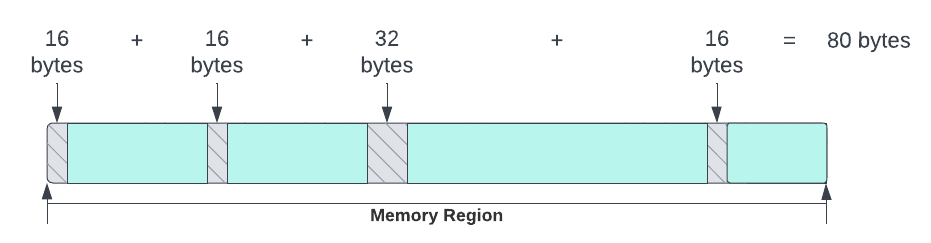
\includegraphics[width=0.8\textwidth]{figures/external_fragmentation.png}
    \caption{A memory region containing several allocated blocks with unused space in between them. Although the total sum of the unused portions is large, a request of more than 32 bytes cannot be fulfilled.}
    \label{fig:external_fragmentation}
\end{figure}

Managing and reducing fragmentation is crucial in optimising memory usage for long-running programs, as excessive fragmentation can impede the system's ability to efficiently allocate contiguous blocks of memory for new objects.

%%% Local Variables:
%%% mode: latex
%%% TeX-master: "main"
%%% End:
